
\chapter{多核操作系统可扩展性分析与建模}

本节将介绍在现代AMD64多核处理器上造成操作系统可扩展性瓶颈的原因。值得注意的是本毕设只考虑由于多核CPU核间通讯开销造成的操作系统性能退化,
一下讨论均忽略系统中其他子系统(如I/O子系统)造成的性能瓶颈。

在造成Linux等现有OS在16核以上多核系统上可扩展性问题的各种因素中,一个核心原因是CPU核间数据共享及其竞争。这种竞争体现在多个方面:

\begin{itemize}
\item 通过原子操作指令(x86中的Lock前缀)修改内核对象的引用计数
(reference count)。由于在x86等体系结构中,一般有已经保证各个核之间的Cache一致性,多个核上使用原子操作修改同一内存地址时,这将迫使
CPU执行Snoop Protocal协议(如在Intel处理器中的QuickPath Interconnect)。在AMD和Intel处理器上Snoop Protocal的复杂度为$O(n)$\cite{intelquickpath},
其中$n$为CPU核数。
当系统中CPU核数增加,各个核上的内存请求将被串行化,这可能会成为操作系统的瓶颈;
\item 通过锁操作控制共享数据访问。为了保证内核中数据结构的一致性,内核需要使用不同粒度的锁保护关键代码段;
\item 通过LAPIC等硬件实现由软件发起的处理器间中断(Interprocessor Interruption)带来的高昂的核间通讯代价。如在多核AMD64系统上,IPI通常被用于发起
TLB无效化请求。
\end{itemize}

下面,我们将使用Linux中虚拟内存子系统作为例子,分析提高操作系统在多核硬件上的可扩展性的重要性和挑战性。

\section{Linux中虚拟内存子系统案例分析}

mmap和munmap两个系统调用是Linux虚拟内存子系统中使用最频繁的系统调用之一,但是对于每个进程,Linux使用一个大锁来保护其VMA结构体:

\begin{lstlisting}
/* Linux 3.9.2 mm/utils.c */
down_write(&mm->mmap_sem);
ret = do_mmap_pgoff(file, addr, len, prot, flag, pgoff,
		&populate);                        
up_write(&mm->mmap_sem);                               
\end{lstlisting}

如上面代码所示,Linux中对同一进程的mmap调用都加上了锁,实际上串行化了所有虚拟内存分配操作,这可能成为频繁调用这两个系统调用分配和释放内存的
多线程应用的瓶颈。事实上,现在Linux中对两个系统调用的实现完全不具有多核可扩展性。事实上,我们可以使用一个简单的程序来验证Linux中mmap系统调用的可扩展性问题:

\begin{lstlisting}
static void *  thread_mmap(void *arg){                                                                                               
        int id = (int)arg;                                                                      
        int c = 0, i;                                                                         
        for(i=0;i<COUNT;i++){                                                                   
                int l = 4096 * (rand() % 5 + 1); 
                void *t = mmap(NULL, l, PROT_WRITE|PROT_READ, 
                      MAP_PRIVATE|MAP_ANONYMOUS, -1, 0);
                assert(t != MAP_FAILED);                                                        
                c++;                                                                            
        } 
        counter[id] = c;                                                                        
        return NULL;                                                                            
}                                                                                               
                                                                                                
int main(int argc, const char* argv[]) {                                                                                               
        /* ... */
        for(i=0;i<threads;i++)
                pthread_create(th+i, NULL, thread_mmap, (void*)i);                              
                                                                                                
        for(i=0;i<threads;i++)                                                                  
                pthread_join(th[i], (void**)&res); 
        /* ... */
}                                                                                                                          
\end{lstlisting}

在上面的程序中,用mmap系统调用多次向操作系统申请空闲的虚拟地址空间。由于同一进程的多个线程共享同一个地址空间(即同一VMA结构体),这在多核系统上将造成mm->mmap\_sem锁的饱和竞争情况,测试结果如图\ref{fig:mmap_test}所示。应该注意的是,我们调用mmap时使用了MAP\_PRIVATE和MAP\_ANONYMOUS标志,并且不指定addr参数申请固定的虚拟内存地址,操作系统应该有最大的自由度选择适当的虚拟内存区域避免VMA操作的竞争。但从测试结果可以看出,当CPU核数增多时,每秒执行的mmap次数反而降低。这符合Linux代码中VMA结构上由于内核中锁竞争造成应用程序严重性能瓶颈的预期。但是,下面我们将通过对Posix系统调用接口中mmap/munmap和缺页中断的建模,并通过符号执行技术证明Linux中对非重叠区域上VMA全局进程锁是不必要的。

\begin{figure}[ht]
\begin{center}
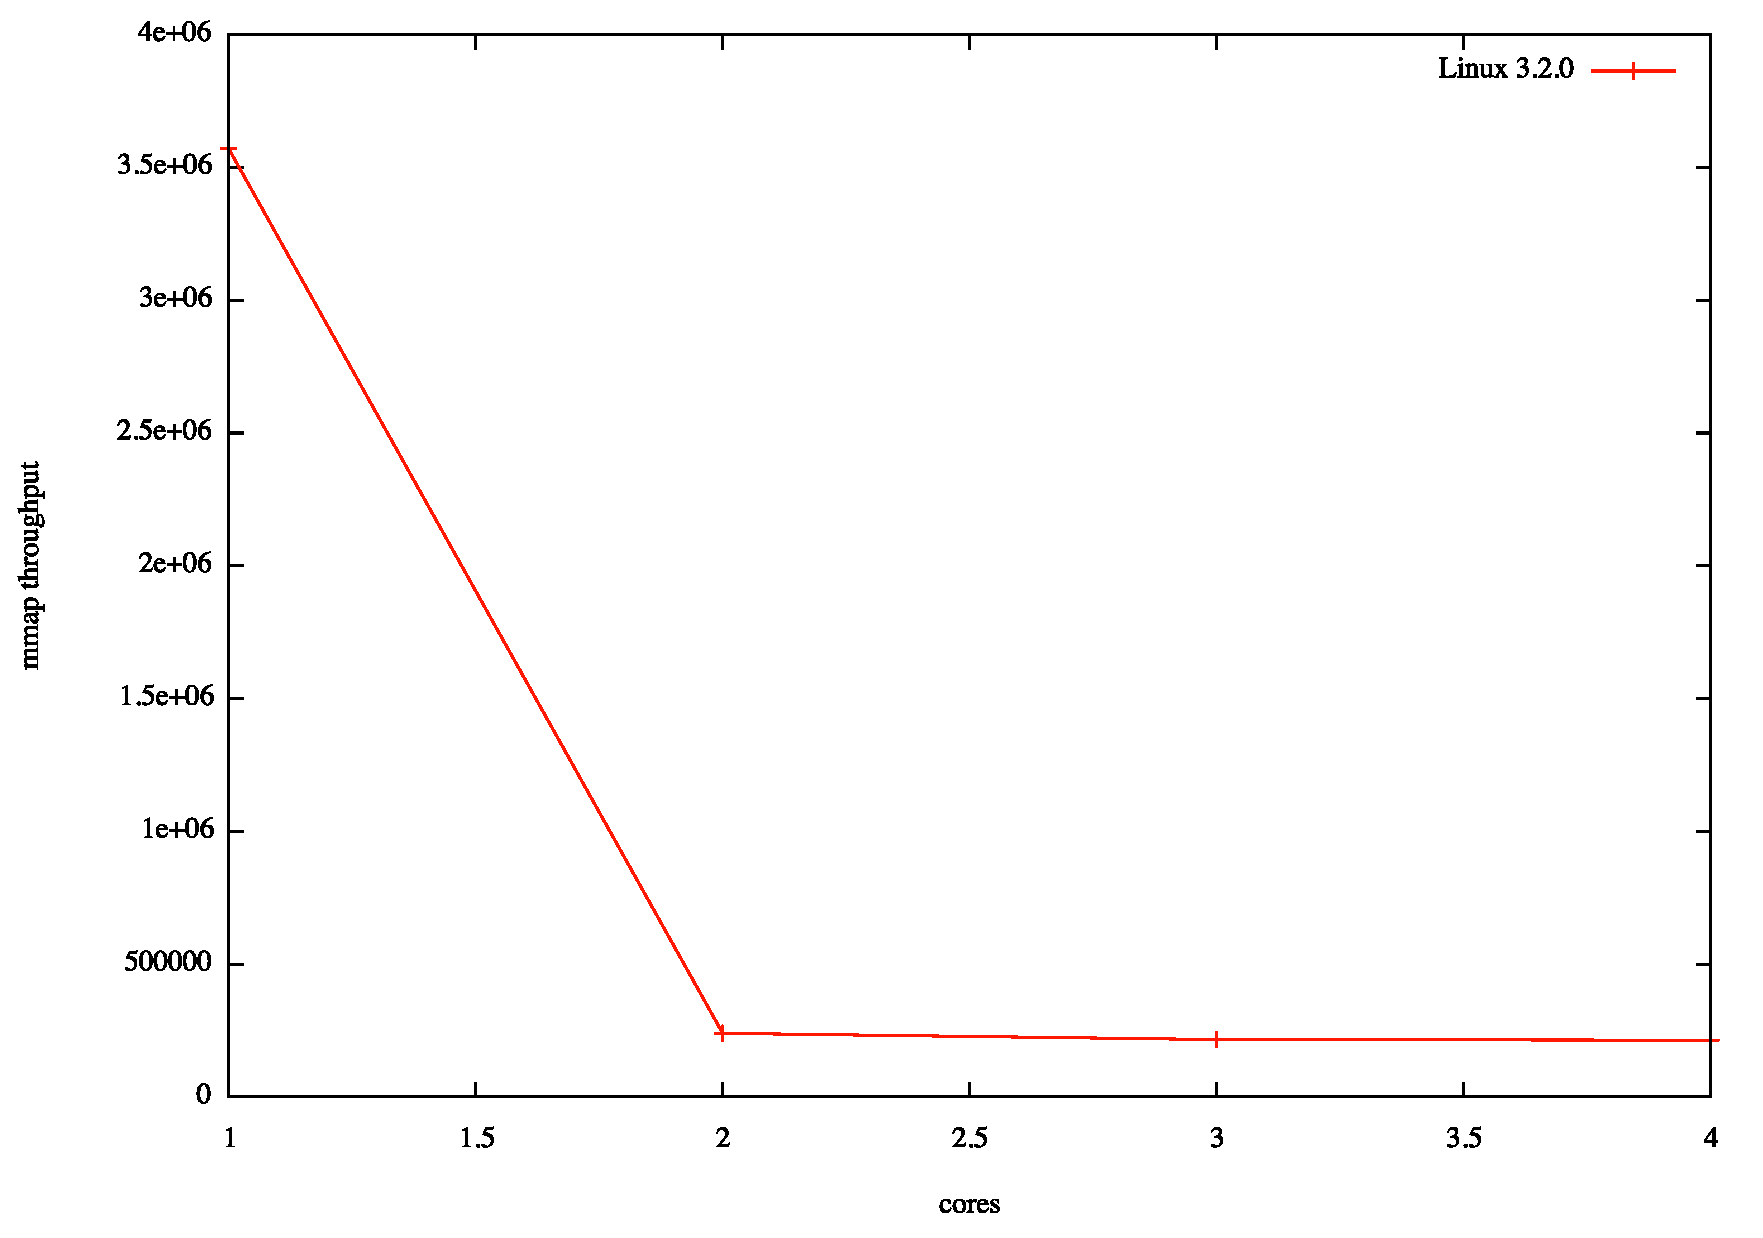
\includegraphics[width=0.7\textwidth]{figures/mmap_test.pdf}
\end{center}
\caption{多核系统mmap饱和测试}
\label{fig:mmap_test}
\end{figure}

\section{可交换性原理}

从上面的案例分析中我们可以知道,现有操作系统内核的部分子系统在多核硬件上表现不如人意。但是,在做出具体可扩展性优化之前,有必要充分论证这种优化的存在性。例如,根据Posix系统调用规范,open系统调用必须返回当前进程中最小的未被使用的文件描述符。如果严格遵循这种规范,open接口规范本身就无法做到并行可扩展,因为实现者必须串行化这些调用来获得最小的文件描述符。另一方面,对于mmap等调用,Posix标准并没有对匿名页返回地址做任何要求(用户指定除外),事实上,造成VM操作在Linux、FreeBSD上可扩展性问题的原因是他们使用了红黑树或伸展树来管理虚拟内存映射\cite{radixvm:eurosys13},这类数据结构需要一个大锁来保护其内部状态(如红黑树的内部节点)的一致性,即使VM操作涉及的是两个不相关的叶子节点。

为了解答这个问题,受到编译器优化技术的启发,有研究者提出了一种在系统接口(如Posix规范)中发现可扩展潜能的方法\cite{commuter:2013}。他们称之为``可交换性法则":只要两个操作的顺序可以交换,那么就可以用多核可扩展的方式实现这些操作。其中的原理是,如果两个操作可以交换(不影响操作结果,因此调用者无法分辨它们执行的顺序),那么他们就可以用不造成读-写冲突的方式实现。

根据这条规则,可以认为Syscall的可交换性在一定程度上等价于Syscall的多核可扩展性。
直观理解,当两个Syscall在一定条件下可交换,意味着他们没有数据相关性,通过某种实现可以避免多核CPU对二三级高速缓存的竞争(Cache
Contention),因此可以达到线性加速比(Perfect Scalability)。

理论上,为了发现系统调用可交换条件,需要遍历Syscall实现中的所有条件
分支,这可以用符号执行技术实现。但是真实Syscall实现过于复杂,
我们可以通过归纳Posix标准中对某个Syscall语义的要求,用简化
的模型(Model)描述此语义要求。

基于这条规律,我们提出了基于模型验证(model
checking)和符号执行的方法,求解Posix标准中系统调用的可交换条件。并尝试了使用KLEE\cite{Cadar:2008:KUA:1855741.1855756}解决问题符号执行的问题。

\section{简单建模例子 \pozhehao 引用计数}
本小结使用一个简单的例子,说明接口建模、交换性求解的整个过程。

引用计数器是跟踪对象生命周期的一种常用编程范式。在操作系统的关键数据结构(如共享物理页管理,VMA结构体,inode结构体等)中,都使用了引用计数器来跟踪这些对象的共享情况,当引用计数变为零时及时删除对象占用的内存,防止内存泄露。Linux等系统中,通常使用atomic\_t类型记录对象的引用计数:

\begin{lstlisting}
/* linux 3.9.2 include/linux/fs.h */
struct inode {                            
    /* ... */
    u64                     i_version;   
    atomic_t                i_count;     
};
\end{lstlisting}

正如本章开头所述,使用原子操作不利于操作系统的多核扩展。直观分析,若引用计数的值足够大,随便调换原子加减操作的次序并不会改变程序的运行结果,因此使用某种引用计数器计数,可以在多核上达到较好的可扩展性。
下面我们将对这种简单的引用计数器建模,使用符号执行技术发现其扩展性潜能,说明这种方法的可行性。

我们把引用计数器上的操作(API)抽象为个函数:
\begin{enumerate}
\item counter\_add
\item counter\_dec
\item counter\_iszero
\end{enumerate}

考虑计数器加一和减一操作,使用C编写对应的模型:

\begin{lstlisting}
void counter_add(struct state *counter)
{                                      
        counter->c ++;                 
}                                      
void counter_sub(struct state *counter)
{                                      
        if(counter->c>0)               
                counter->c --;         
        if(counter->c == 0)            
                counter->free = 1;     
} 
\end{lstlisting}


\section{虚拟内存管理子系统的建模}

近年来,随着SMT求解器,如STP、MathSAT、Z3的进步,为符号执行和模型验证方法提供了越来越强大的后端支持,使对操作系统等一类高复杂度软件的形式化验证成为了可能。事实上,在OSDI近年的会议上,已有多项针对OS中文件系统子系统的建模工作\cite{radixvm:eurosys13}\cite{Yang:2006:UMC:1189256.1189259},但他们的主要着眼点在使用模型验证和符号执行手段分析现有文件系统的Bug和错误上。
在文件系统方面,MIT的Commuter\cite{commuter:2013}的一个创新点是把符号执行与可交换性法相结合,提出了在Posix文件系统API规范中发掘多核可扩展机会的方法。

我们希望把Commuter的思路进一步扩展到OS的其他子系统,通过为操作系统虚拟内存管理、进程管理子系统进行建模,提供一种可以跨OS子系统分析操作系统接口多核可交换性/可扩展性的方法。

首先,我们认为对虚拟内存子系统系统调用建模发现潜在的可扩展性因素越来越有必要。正如文章\cite{radixvm:eurosys13}所说,在多核系统上OS的VM子系统对于VM密集型应用(如Java垃圾回收器)上已经成为了瓶颈,大大限制了多线程编程模型的多核可扩展性。通过建模发现Posix
VM API中可扩展性的潜能,以此为基础提出更好的Posix系统调用实现方式。

另一方面,我们认为对OS的虚拟内存管理系统/管理系统建模是一项比对文件系统建模更有挑战性的工作,有如下两个原因。

第一,文件系统主要以数据结构的更新逻辑为主,对open、read等系统调用建模时可以把底层硬件(如磁盘)抽象为数组。因此已有工作对文件系统相关系统调用都没有考虑硬件的影响。而对虚拟内存子系统建模时,必须考虑硬件缺页中断等硬件相关的影响。

第二,实际操作系统中,对虚拟内存和进程的管理设计大量共享可变数据结构(shared
mutable),如fork系统调用对物理页的写时复制(Copy-on-Write)策略,信号量的共享等。这种特性与Z3等SMT求解器以函数式语法描述程序约束条件的情况相对立,使得可交换性条件求解变得困难。

下面我们以操作系统中虚拟内存管理(Virtual Memory)子系统为例,介绍简化的Posix系统调用API接口和中断处理例程的建模方法。
在OS的虚拟内存管理子系统中,有两个最重要的系统调用:mmap和munmap。与文件系统建模不同的是,为了相对完整地描述虚拟内存子系统的行为,模型中还必须包括VM子系统对缺页异常(pagefault
handler)的处理例程。[XXX 如何扩展论述?]

对于内存管理子系统,我们把操作系统对程序的接口分成两类:
\begin{enumerate}
\item OS提供给用户态程序的系统调用接口,如mmap/mumap系列函数;
\item 用户程序访问硬件页表发生缺页中断时,操作系统根据虚拟地址区域的元数据(如Linux中的VMA结构体)填写缺失的硬件页表项。对于由软件填充TLB的体系结构,如MIPS,也可以通过软件模拟页表的方法实现类似功能。
\end{enumerate}

在编写操作系统的过程中,我们发现上述两类操作系统接口可以统一建模。由于在x86\_64(或其他大部分体系结构中)缺页异常属于同步异常\cite{intelsys},可以把读写缺页看做普通系统调用,通过添加如下两个虚拟系统调用对缺页进行建模:

\begin{verbatim}
void mem_write(pid, addr, value)
word mem_read(pid, addr)
\end{verbatim}

\subsection{系统调用建模}

\subsection{中断建模}

\section{基于模型的可交换性求解}

\subsection{基本算法}

\subsection{使用KLEE求解模型}
KLEE是基于LLVM
bytecode的符号执行引擎。KLEE已经被广泛地应用在文件系统建模,大型开源软件(如GNU
coreutils)漏洞查找\cite{Cadar:2008:KUA:1855741.1855756}等方面。KLEE中使用了一种简单的方法来避开指针和Heap对象约束求解的困难:记录指针可能引用的对象集合,在指针被dereference的时候,如果此指针可能指向N个对象,则fork出N个状态并进入调度队列,之后再继续进行符号执行。状态之间,KLEE使用写时复制(Copy-on-Write)的方式管理内存。有研究者对这种方法做扩展。


\subsection{进一步讨论}
Separation Logic是对Hoare
Logic的一种扩展,理论上可以用于对使用共享可变数据结构(如Heap上分配的对象)的命令式程序做推导[7]。考虑如下程序:

【XXX 多数sep logic论文使用reverse list。我们应该用OS中单向链表使用的例子】

形式上Separation Logic定义了Separating Conjuction运算符:P *
Q,表示程序的堆(Heap)可分割为两个独立的堆H1、H2,在H1上命题P成立,在H2上命题Q成立。直观上,通过Seperating
conjuction运算符和相关推理规则,简化了Heap上包含共享数据结构程序约束的描述。然而,文章[7]中并未给出Separation
logic的判定过程(decision
procedure),Z3等SMT求解器未支持此类逻辑的可满足性判定。但是,对于separation
logic的一些特殊情况,学界已经提出了相关的判定过程。例如,对于操作系统中的使用最频繁的链表结构,文章[9]提出了求解下面形式约束的算法,并在Z3
SMT求解器中实现:

[公式 XXX -> xxxxx]
其中XXX是xxx


\section{小结}
XXX TODO
